\section{Correctness and Performance}
\label{correct}

We now consider some correctness and performance issues raised by the use
of Coccinelle.

\subsection{Correctness}

For the traditional uses of Coccinelle, for bug finding and collateral
evolutions, a developer runs Coccinelle once on a code base, checks and
possibly adjusts the results, and submits a patch upstream for review by
kernel maintainers.  The patch is integrated into the Linux kernel just
like a manually generated patch, and Coccinelle is no longer involved.

The use case for backports is rather different.  Here, the developer
typically starts with a collection of patches, reflecting the result of
backporting a number of drivers by hand.  The developer then generalizes
the existing patches into a semantic patch, which is then applied every
day, as linux-next and the various stable kernels evolve.  In this context,
manually studying each result is not practical, and would likely not be
reliable.  Still, it is necessary to account for the possibility of errors,
either in the semantic patch definition or in Coccinelle itself.  Indeed,
some improvements to Coccinelle were required to enable its use for
backporting, such as improving the support for adding \#ifdefs around
complete function definitions.

To check the correctness of the result of Coccinelle, we exploit the
existence of manually developed patches that perform the desired
transformation.  Specifically, we have developed a simple tool that applies
the manually developed patches and the semantic patches to separate copies
of the Linux kernel source code, and then checks that the results are
equal.
%
After applying the semantic patches to a possible target release and
comparing the result with that of applying the manually written backport
patches, we were surprised to find that the semantic patches produced more
code changes.  Indeed, the functionalities backported by the semantic
patches occur in drivers that, while they are integrated on Linux
backports, are not yet enabled for older kernels, as they require
backporting of more collateral evolutions. A semantic patch transforms all
code that exhibits the specified pattern, and thus generalizing a backport
with Coccinelle can extend that backport to more drivers. Once all of the
collateral evolutions required by a particular driver for a given kernel
have been implemented, then that driver can be enabled for use on that
kernel.  When all required collateral evolutions to support a given kernel
have been addressed with Coccinelle, then new drivers can be backported to
that kernel fully automatically.

%% Since git is prevalent on the target directories where we typically
%% want to do changes I just use git, and what I do is apply the legacy
%% patch first, commit that. Then I apply the inverse of the patch but do
%% not commit that, and then I apply the SmPL patch. All + stuff is
%% things that is extra, all - stuff is stuff that is removed. This is
%% how I found out about the different collateral evolution that we
%% tugged along into the original patch series.


\subsection{Performance}

Each day, the Linux kernel backports project generates and compile tests
backport releases for all supported kernels, of which there are currently
18.  Generation for all of them takes around 2 minutes on our 32-core
machine, and compile testing of the 18 resulting patched kernels takes 40
minutes of real time, comprising 1086 minutes of user time and 139 minutes
of system time.  Given the long compilation time, it is important to
minimize the time for generating backports.  Several solutions were
explored to avoid the use of Coccinelle overwhelming the backporting time.
Figures \ref{num_patches} and \ref{small_num} relate the backport
generation time to the number of supported kernels, patches, and resulting
backported drivers for recent kernels.

%% real    40m15.411s
%% user    1085m54.776s
%% sys     139m23.312s

%% This is across these 18 kernels (including v3.17, but obviously we
%% should skip that):

%% 1   3.0.101             [  OK  ]
%% 2   3.1.10              [  OK  ]
%% 3   3.2.62              [  OK  ]
%% 4   3.3.8               [  OK  ]
%% 5   3.4.103             [  OK  ]
%% 6   3.5.7               [  OK  ]
%% 7   3.6.11              [  OK  ]
%% 8   3.7.10              [  OK  ]
%% 9   3.8.13              [  OK  ]
%% 10  3.9.11              [  OK  ]
%% 11  3.10.54             [  OK  ]
%% 12  3.11.10             [  OK  ]
%% 13  3.12.27             [  OK  ]
%% 14  3.13.11             [  OK  ]
%% 15  3.14.18             [  OK  ]
%% 16  3.15.10             [  OK  ]
%% 17  3.16.2              [  OK  ]
%% 18  3.17-rc3            [  OK  ]


%% For this, the project uses a
%% 32-core server donated by HP, SUSE and the Linux Foundation, having 236 GiB
%% RAM.  The project uses a /pub/mem tmpfs, allowing it to have the upstream
%% Linux kernel git tree and the stable kernel git tree,\footnote{The
%%   linux.git and linux-stable.git git trees from kernel.org, respectively.}
%% the backport patches and the compat library, and all of the generated code
%% in RAM. Compilation tests are all performed in RAM.  Prior to the use of
%% Coccinelle, the compilation time dominated the daily tasks involved in
%% backporting.  Applying a semantic patch involves parsing and processing
%% source code, and is thus much more expensive than simple line-by-line patch
%% application.  Several solutions were explored to avoid the use of
%% Coccinelle overwhelming the backporting time.

\begin{figure}
\[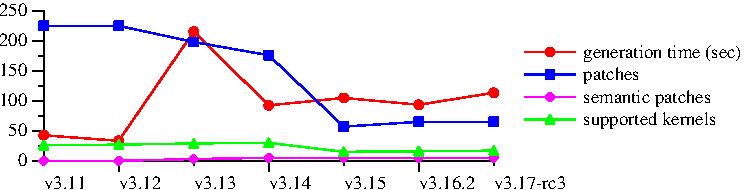
\includegraphics[width=\linewidth]{patchtimes.pdf}\]
\caption{Generation time compared to number of patches, semantic patches,
  and supported kernel versions}
\label{num_patches}
\[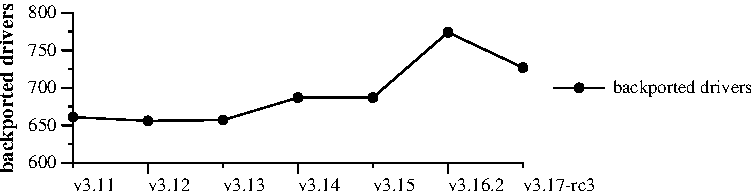
\includegraphics[width=\linewidth]{small_supported.pdf}\]
\caption{Number of backported drivers, for recent kernels}
\label{small_num}
\end{figure}

As a first try, in v3.13, all of the semantic patches were concatenated and
run in a single thread, much like the application of standard patches.  In
a uniprocessor environment, this avoids the cost of starting up Coccinelle
for each semantic patch.  This solution, however, does not exploit the
parallelism inherent in applying a single specification to the hundreds of
drivers supported by the backports project, and we see a high generation
time in Figure \ref{num_patches} for v3.13.  Coccinelle currently supports
static parallelism via an external script that starts up $n$ instances of
Coccinelle and causes each of them to process $1/n$ of the files in the
code base.  Performance can further be improved by instructing Coccinelle
to use index information, precollected by a tool such as
glimpse,\footnote{http://webglimpse.net/.  As a side effect of this work,
  the first author convinced the developers of glimpse to release glimpse
  as open source.} to identify the subset of files that may be relevant to
a given semantic patch.  With these two optimizations, semantic patch
support can be less expensive than sequential application of the
corresponding patches.  For example, for v3.26.2, the number of supported
drivers increases significantly (Figure \ref{small_num}), but the generation
time actually slightly goes down.  Currently, we are exploring the
integration of parallelism into Coccinelle itself using the OCaml library
Parmap \cite{Danelutto:12}, which provides dynamic scheduling.  Preliminary
tests suggest that this will improve CPU utilization and yield further
performance improvements.

%% \subsection{Coccinelle Parallelizing improvements}

%% The backports project ended up fine tuning usage of Coccinelle
%% with sensible arguments and managing Coccinelle's current parallelism
%% support using Python. The script was generalized for regular
%% kernel development and is now merged on Coccinelle development
%% git tree. It is used as follows:

%% \begin{lstlisting}[language=bash]
%% pycocci foo.cocci drivers/
%% \end{lstlisting}

%% This script causes Coccinelle to make changes in place in the source code
%% (Coccinelle option {\tt -{}-in-place}, it is parallelized, and a number of
%% other sensible command-line arguments are provided if one wants to apply
%% rules broadly. In the future, Coccinelle will be modified to use the OCaml
%% Parmap library for integrated parallelism support. In order to help make
%% Coccinelle run faster software index utilities can be used, glimpse is one
%% option, another is idutils. Glimpse is unfortunately not FOSS. By default
%% Coccinelle relies on its own grep implementation to search for tokens.

\subsection{Further improvements: a needle in a haystack}

Coccinelle applies the rules of a semantic patch in order, from first to
last, with any changes specified by a rule being performed as soon as
the rule is matched.  This can lead to extra matching and undesired
modifications if rules that perform generic transformations are placed at
the beginning of a semantic patch.  As an example, consider the following
rule that begins a semantic patch for backporting PCI drivers:

\begin{lstlisting}[language=diff]
@ simple_dev_pm depends on module_pci @
identifier ops, pci_suspend, pci_resume;
declarer name SIMPLE_DEV_PM_OPS;
declarer name compat_pci_suspend;
declarer name compat_pci_resume;
@@
+compat_pci_suspend(pci_suspend);
+compat_pci_resume(pci_resume);
SIMPLE_DEV_PM_OPS(ops, pci_suspend, pci_resume);
\end{lstlisting}

%% In the following 419 comes from searching for SIMPLE_DEV_PM_OPS, and 61
%% comes from additionally looking for the declaration and initialization
%% of a pci_driver structure.  See misc/pcipm.cocci on palace.

\noindent
This rule collects some information from each {\tt
  SIMPLE\_\-DEV\_\-PM\_\-OPS} structure, and introduces some PCI-specific
calls from the compat library.  The rule applies to every {\tt
  SIMPLE\_\-DEV\_\-PM\_\-OPS} declaration, and is not specific to PCI
drivers in any way.  Not only does it transform code that should not be
transformed, it also can potentially have a significant performance impact.
In the linux-next of October 15, 2014, there are 419 files that contain a
{\tt SIMPLE\_\-DEV\_\-PM\_\-OPS} declaration, while only 61 of these are
PCI drivers.  All of these extra files will be parsed and (unnecessarily)
transformed if the semantic patch is written in this way.

A solution is to add a rule that matches against some other more specific
term that must be present if any transformation is to be performed.  Other
rules can then depend on the success of matching this rule.  Essentially,
this rule acts as a ``needle in a haystack'' to find the source files
where the transformation is actually relevant.  In this particular case, we
observe that PCI drivers contain a {\tt MODULE\_\-DEVICE\_\-TABLE}
declaration with {\tt pci} as the first argument. We thus add the following
rule at the beginning of the semantic patch:

\begin{lstlisting}[language=diff]
@ module_pci @
declarer name MODULE_DEVICE_TABLE;
identifier pci_ids;
@@
MODULE_DEVICE_TABLE(pci, pci_ids);
\end{lstlisting}

The {\tt SIMPLE\_\-DEV\_\-PM\_\-OPS} rule can now be declared to depend on
the rule {\tt module\_\-pci}, ensuring that it is only applied to PCI
drivers:

\begin{lstlisting}[language=diff]
@ simple_dev_pm depends on module_pci @
identifier ops, pci_suspend, pci_resume;
declarer name SIMPLE_DEV_PM_OPS;
declarer name compat_pci_suspend;
declarer name compat_pci_resume;
@@
+compat_pci_suspend(pci_suspend);
+compat_pci_resume(pci_resume);
SIMPLE_DEV_PM_OPS(ops, pci_suspend, pci_resume);
\end{lstlisting}

The final rule to perform the backport uses metavariables that are
defined by the previous one, and thus by that rule's dependence will also
only be applied to PCI drivers:

\begin{lstlisting}[language=diff]
@@
identifier backport_driver;
expression pm_ops;
fresh identifier backports_pci_suspend = simple_dev_pm.pci_suspend ## "_compat";
fresh identifier backports_pci_resume = simple_dev_pm.pci_resume ## "_compat";
@@
struct pci_driver backport_driver = {
+#if (LINUX_VERSION_CODE >= KERNEL_VERSION(2,6,29))
	.driver.pm  = pm_ops,
+#elif defined(CONFIG_PM_SLEEP)
+	.suspend	= backports_pci_suspend,
+	.resume 	= backports_pci_resume,
+#endif
};
\end{lstlisting}

%% \subsection{Coccinelle is precise}

%% One of the benefits of Coccinelle is that its less prone to errors.
%% Indeed, previous experience has shown that manually backporting complex
%% collateral evolutions is error prone. In this section we'll provide an
%% example of how a rule will only modify the data structure specified, even
%% if similar data structures exist with similar member names.\footnote{The
%%   code presented in this section can be obtained and tested at:
%%   https://github.com/mcgrof/netdev-ops.git, with the command sequence {\tt
%%     make test1}, {\tt git checkout -f}, {\tt make test2}.}

%% Consider the following code: \jl{Is something missing in the include?}

%% \begin{lstlisting}[language=C]
%% #include

%% struct net_device_ops {
%% };

%% struct net_device {
%% 	struct net_device_ops *netdev_ops;
%% };

%% struct bubble_ops {
%% };

%% struct bubbles {
%% 	struct bubble_ops *netdev_ops;
%% };

%% static struct net_device_ops my_netdev_ops = {
%% };

%% static struct bubble_ops my_bubble_ops = {
%% };

%% static struct parent {
%% 	struct net_device *dev;
%% 	int b;
%% };

%% static struct parent_usb {
%% 	struct net_device *net;
%% 	int b;
%% };

%% int main(void)
%% {
%% 	struct parent *p = malloc(sizeof(struct parent));
%% 	struct parent_usb *p_usb = malloc(sizeof(struct parent));
%% 	struct net_device *dev = malloc(sizeof(struct net_device));
%% 	struct bubbles *bubble = malloc(sizeof(struct bubbles));

%% 	dev->netdev_ops = &my_netdev_ops;
%% 	bubble->netdev_ops = &my_bubble_ops;

%% 	free(dev);
%% 	free(bubble);
%% 	free(p);
%% 	free(p_usb);

%% 	p->dev = dev;
%% 	p->dev->netdev_ops = &my_netdev_ops;
%% 	p_usb->net->netdev_ops = &my_netdev_ops;

%% 	return 0;
%% }
%% \end{lstlisting}

%% The following semantic patch will modify both {\tt net\_\-device} structures
%% and {\tt bubbles} structures, which is undesirable.

%% \begin{lstlisting}[language=diff]
%% @@
%% expression dev;
%% expression ops;
%% @@
%% -dev->netdev_ops = ops;
%% +netdev_attach_ops(dev, ops);
%% \end{lstlisting}

%% \noindent
%% To address this problem, SmPL makes it possible to be explicit about the
%% types of the data structures that should be modified:

%% \begin{lstlisting}[language=diff]
%% @@
%% struct net_device *dev;
%% struct net_device_ops ops;
%% @@
%% -dev->netdev_ops = &ops;
%% +netdev_attach_ops(dev, &ops);
%% \end{lstlisting}

%% \noindent
%% This refined semantic patch will only make changes to structures of type
%% {\tt net\_\-device}.
